\subsection{Spectrometers and Detectors}\label{sec:HRS}

The Hall A high resolution spectrometers (HRS) at
Jefferson Lab consist of a pair
of identical spectrometers of QQDQ design,
together with detectors for detecting the 
scattered particles \cite{A-NIM}.
The spectrometer and their standard detector 
package served to select for and to 
measure the kinematics quantities ($x, Q^2$)
while suppressing backgrounds originating
from the target.

\par
The spectrometers are designed to have a
large acceptance with excellent 
resolution ($\Delta E / E \sim 10^{-4}$)
and absolute accuracy
in the reconstructed
four--vectors of the events and, 
of less relevance for our experiment,
precise normalization of the cross section.
To measure $Q^2$ with sufficient accuracy
requires good knowledge of the transfer matrix for
the spectrometer to reconstruct events at the
scattering point, as well as
good pointing accuracy for the location of the
spectrometers and precise measurements 
of beam position and angle.
To calibrate the transfer matrix, a 0.5 mm thick 
tungsten plate with an array of pinholes
is inserted in dedicated runs; reconstruction
of the hole pattern determines the matrix.

The scattered rate of electrons and of pions were 
determined by a trigger system
in the HRS described in ~\cite{pvdis_nim}.
This trigger consisted of two scintillator planes, which provided
the main timing trigger, a CO$_2$ gas cherenkov counter and a 
double-layered lead glass 
detector, which both provided particle identification information. 
The standard tracking detector (the vertical 
drift chamber) was turned off during production data 
taking because it may not endure
the expected high event rates. 
During low-rate calibration runs, the tracking detector 
was turned on and the efficiency of the electron trigger 
and the pion rejection could be studied (see ref ~\ref{pvdis:nim}).

The signals for
the gas cherenkov detector and the double-layered lead glass counter
were passed through discriminators and logic units to form 
preliminary electron and pion triggers. 
These preliminary triggers are then combined with the 
scintillator triggers and cherenkov 
signals to form the final electron and pion triggers, which are then 
sent to scalers to record the event counts and form asymmetries.  
Particle identification 
is fulfilled by the use of discriminators for both the lead-glass 
and the cherenkov counters 
and proper settings of their thresholds. 

For HRS the two layers of the leadglass counter are 
called ``preshower'' and ``shower'' detectors, 
respectively. The preshower blocks in the Right HRS 
(the spectrometer located to the right 
side of the beamline when viewed along the beam direction) 
has $48$ blocks arranged in a $2\times 24$ 
array, with the longest dimension of the 
blocks aligned perpendicular to the particle trajectory. For the two blocks
in each row, only the ends facing outward are read 
out by photo-multiplier tubes (PMTs) and 
the other ends of the two blocks were facing each other 
and not read out. Therefore the 
preshower detector had $48$ output channels. All preshower 
blocks were individually wrapped 
to prevent light leak. The preshower and the shower detectors 
in the Left HRS are similar to 
the preshower detector on the Right HRS except that for each 
detector there are $34$ blocks 
arranged in a $2\times 17$ array. The shower detector in the 
Right HRS had $75$ blocks 
arranged in a $5\times 15$ array with the longest dimension 
of the blocks aligned along the trajectory of 
scattered particles. PMTs are attached to each block of 
the Right shower detector on one end only, 
giving $75$ output channels.

The particle identification (PID) was studied at 
low beam currents using 
fbTDC signals along with ADC spectrum
of all detector signals recorded by the standard DAQ. 
Figure~\ref{fig:showerspectrum} shows the preshower vs. shower
signals for group 2 on the Left HRS. A comparsion between no fbTDC cut and with 
cut on the fbTDC signal of the electron wide trigger from this group clearly shows the 
hardware PID cuts.
%
\begin{figure}[!ht]
\hspace*{0.8cm}
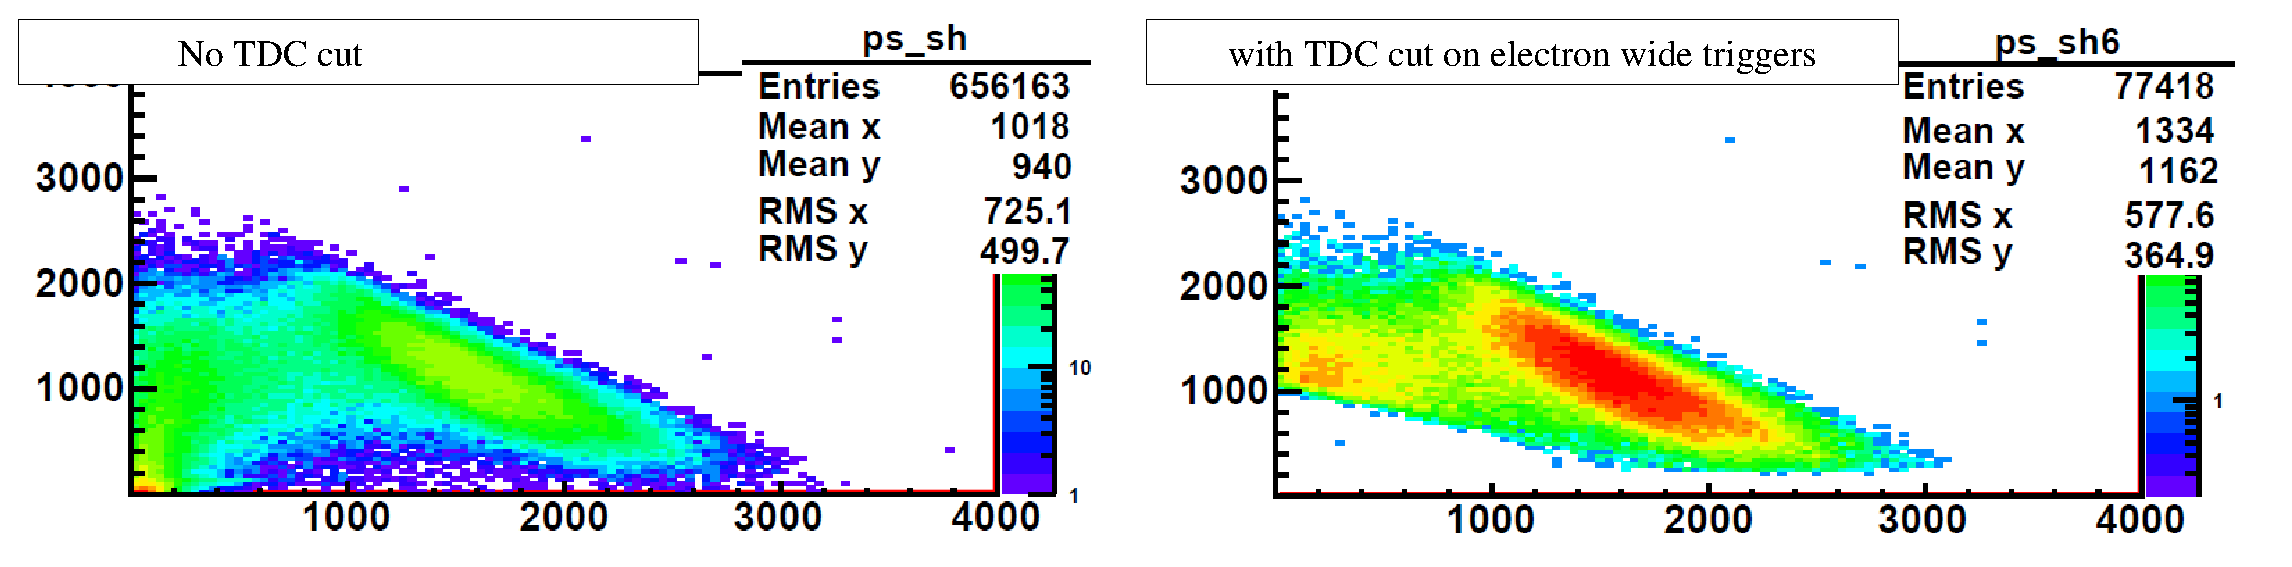
\includegraphics[width=0.9\textwidth]{RM/run_22060_group2_PSvsSH_edit.eps}
\hspace*{-0.2cm}
\caption{Preshower vs. Shower ADC spectrum (sum of 8 blocks each) for group 2 on the Left HRS,
without fbTDC cut (left) and with cut on the group 2 electron wide trigger fbTDC
signal (right). It clearly shows the hardware cuts on the preshower and the total
shower signals, indicating the DAQ is selecting the correct events
as electrons. The cuts can be adjusted by changing the discriminator 
thresholds.
The events near the vertical axis, around ADC channels (200,1000), 
are electrons that deposited energy in overlapping blocks between group 2 and group 1 
(or group 3) and are recorded by the other group.
}
\label{fig:showerspectrum}
\end{figure}


Electron efficiency
and pion rejection factors of the lead glass counter on the Left HRS are 
shown in Fig.~\ref{fig:pidLeft} as functions of the vertical hit position 
of the particle in the preshower detector. PID performance on the Right HRS
is similar.
%
Electron efficiency from wide groups are slightly higher than narrow groups
because there is less event loss due to timing mis-alignment when taking the
coincidence between the preshower and the total shower discriminator outputs.
%
Variations in the electron efficiency across the spectrometer acceptance 
effectively change the kinematics $(Q^2)$ of the measurement. For this reason, 
data were taken daily during the experiment to monitor the DAQ PID performance
and corrections are applied to data. 

Combined with the $\approx 200$ pion rejection factor of the gas cherenkov
counter, the total pion rejection was above $10^{4}$. With the parity violation
asymmetry of pion production being no larger than that of scattered electrons, 
the uncertainty in the final asymmetry results due to pion contamination is
negligible compared to the $3-4\%$ statistical uncertainty.

%%%%%%%%%%%%%%%%
\begin{figure}[!ht]
\hspace*{-0.6cm}
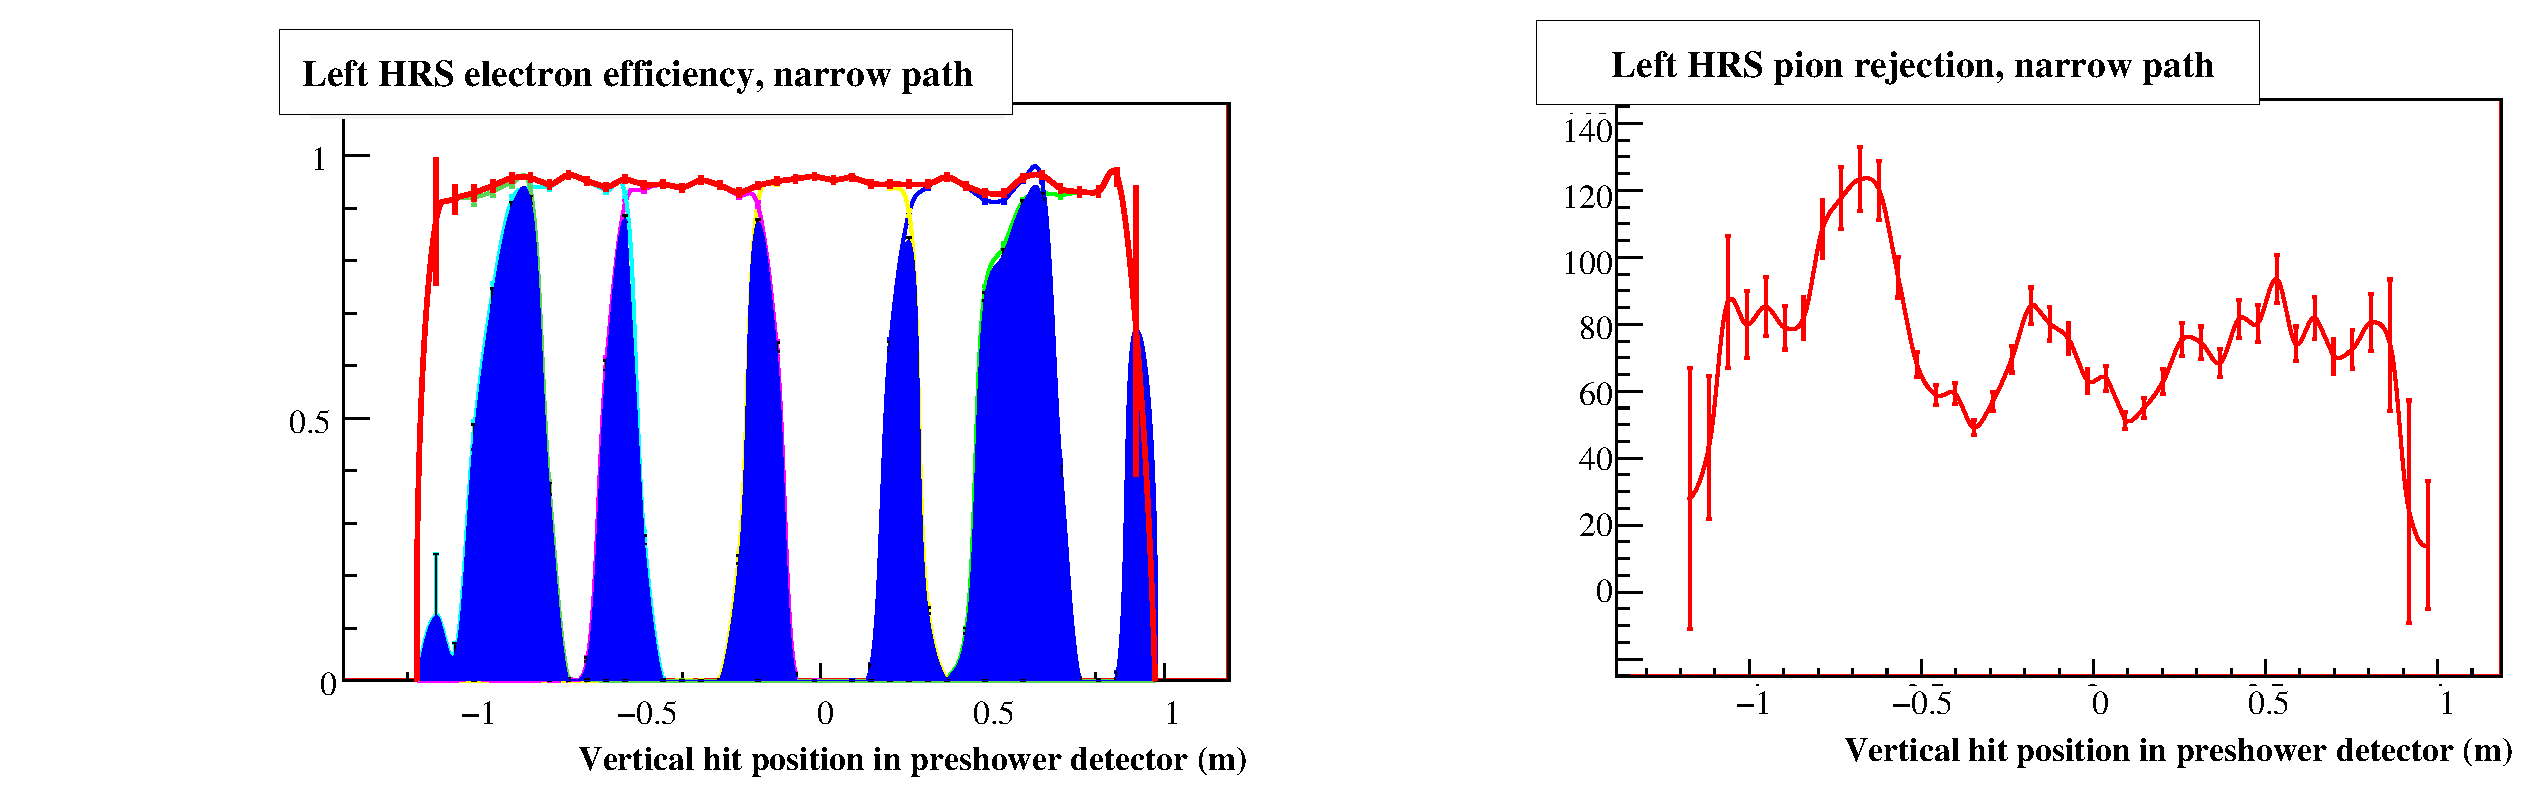
\includegraphics[width=\textwidth,angle=0]{RM/PIDLeft_edit_horizontal.eps}
\caption{Electron detection efficiency (left) and pion rejection factor (right) 
vs. vertical (dispersive) hit position of the particle in the preshower detector 
for the narrow electron triggers in the Left HRS. A one-hour run was used in this 
evaluation.
For electron efficiencies, the total efficiency is shown by the red curve, while blue 
shaded area indicates events that are recorded by the two adjacent groups. 
The average electron efficiency across the detector for this one-hour run
is $(94.626\pm 0.002)\%$ and the averge
pion rejection factor is $75.3\pm 1.1$. The error bars are statistical only.
PID performance for the wide path and the Right HRS are similar.
}
\label{fig:pidLeft}
\end{figure}


